\section{RESULTS}
\label{sec:Res}

We prove the validity of the geometric hints in semantic surface segmentation, and evaluate our method on two widely used datasets: LSUN dataset \cite{zhang2015large} and Hedau dataset~\cite{hedau2009recovering}. 

\subsection{Analysis of Geometric Hints}
\label{sec:ablation}
To explore the benefits of geometric hints for semantic surface segmentation, we train FCNs with or without geometric hints, respectively. 
Their performance are evaluated on the LSUN validation set using pixel error of $\vb{\hat{L}}$, which can be seen in Table~\ref{table:ablation}. To make fair comparisons with \cite{ren2016coarse, dasgupta2016delay}, both of which are built on VGG16, we train an MC-FCN based on VGG16 too. For \cite{ren2016coarse}, we directly apply their trained model to generate $\vb{\hat{L}}$. And for \cite{dasgupta2016delay}, we train an FCN having the same architecture with \cite{dasgupta2016delay}. As revealed by Table~\ref{table:ablation}, with the help of geometric hints, our MC-FCN obtains lower pixel error of $\vb{\hat{L}}$. We further improve the performance by employing ResNet101~\cite{he2016deep} in our FCN. 
Qualitative results are demonstrated in Fig.~\ref{fig:fcn-comparison}. 
Fig.~\ref{fig:fcn-comparison} (a)-(e) show typical good examples. Intuitively, the traditional FCNs are sometimes confused by different surfaces and generate spurious regions due to occlusions and clutters. 
Our method with the geometric hints gets rid of these uncertainties, and attains more accurate semantic surface segmentation. Fig.~\ref{fig:fcn-comparison} (f) depicts an imperfect result, where FCNs tend to be cheated by large truncated wall-like object surfaces, e.g., the bed looks like the floor. This may be the result of ignoring the semantics of the objects. Fig.~\ref{fig:fcn-comparison} (g) is an another challenging case due to clutters, while our MC-FCN produces a relatively clearer result.  

\begin{figure}[!ht]
	\centering 
	\textsc{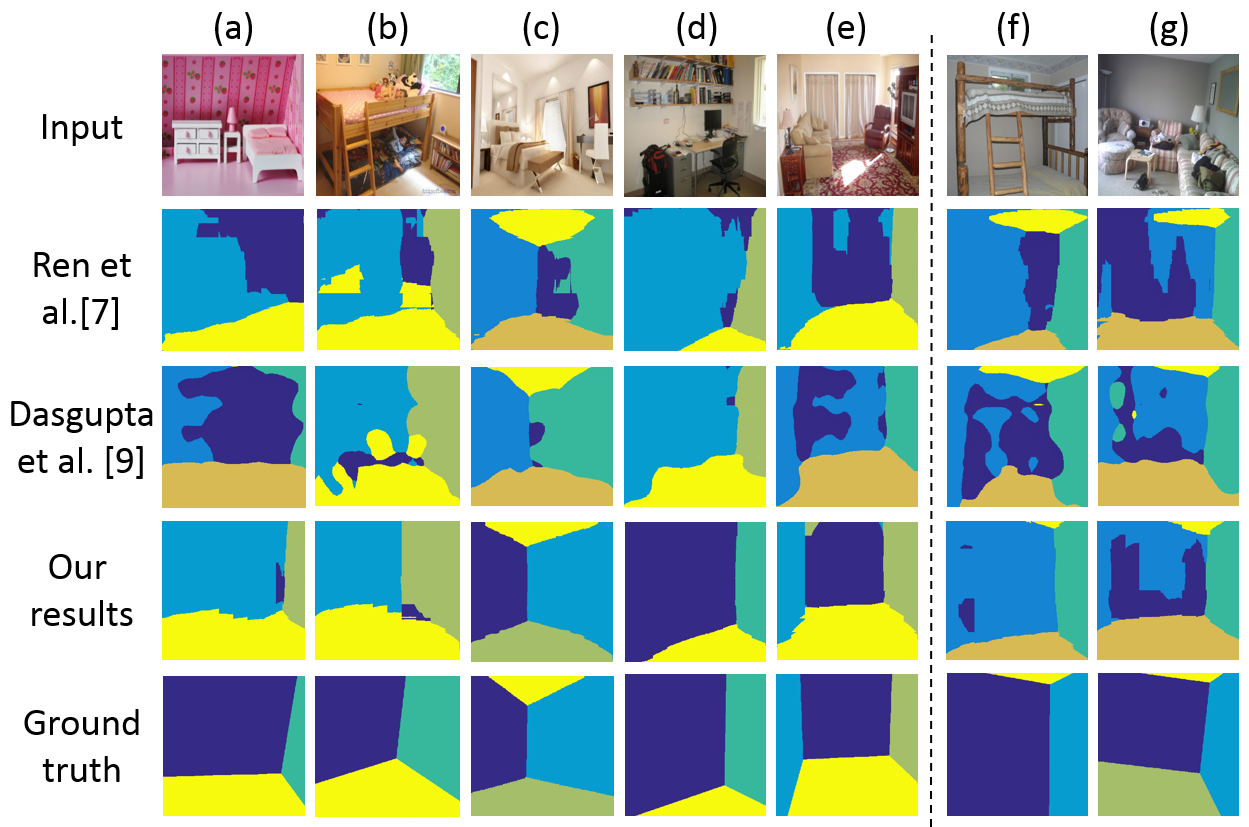
\includegraphics[width=8.5cm]{figure/compare1.png}}
	\caption{Surface segmentation results using different methods. All the networks are built on the VGG16 architecture. Our MC-FCN with geometric hints generates more accurate segmentation, especially for complex environments.}
	\label{fig:fcn-comparison}
\end{figure}

\begin{table}
	\centering
	\begin{tabular}{l|c} 
		\hline
		Network & $\epsilon_{pixel}$ (\%)\\
		\hline
		Ren et al.~\cite{ren2016coarse} & 21.54 \\
		Dasgupta et al.~\cite{dasgupta2016delay} & 15.86 \\  \hline
		MC-FCN (VGG16)  & 14.05 \\
		MC-FCN (ResNet101) & 11.45 \\
		\hline
	\end{tabular}
	\caption{Pixel-wise errors of semantic surface segmentation by different FCNs. By utilizing geometric hints, our proposed MC-FCNs obtain more accurate segmentations. }	
	\label{table:ablation}
\end{table}

\subsection{Results on LSUN Dataset}
\label{sec:LSUN}
We train our multi-channel FCN on the relabeled LSUN dataset released by \cite{ren2016coarse}. The dataset consists of 4000 training images, 394 validation images, and 1000 testing images. 
We extract geometric hints from original images and resize all the images, depth and normal maps to $321\times321$ using bicubic interpolation. 
These three types of data are integrated to train the ResNet101-based multi-channel FCN. 
We evaluate our results using the official toolkit which provides two standard metrics: pixel-wise error and corner error. The pixel-wise error is computed by counting the percentage of pixels that are mismatched. The corner error is computed by calculating the Euclidean distance between predicted corners and corresponding ground truth corners.

We summarize the performance on the test set of LSUN in Table~\ref{table:comparison-lsun}. Qualitative results are displayed in Fig.~\ref{fig:qualitative}. Our approach outperforms traditional methods \cite{hedau2009recovering} and most neural network based methods~\cite{mallya2015learning,zhang2017learning,dasgupta2016delay,ren2016coarse,LeeRoomNet17} on both metrics. 
%
Besides, when training the FCN, Zhao et al.~\cite{zhao2017physics} formulate the room layout using boundaries among semantic surfaces, while we formulate the room layout using the five semantic surfaces, as \cite{dasgupta2016delay} does. 
These two representations may have different application prospects in the future. For example, when a home robot wants to locate itself while it moves, the semantic boundaries are not always available. 
Our method may also be an inspiration for other surface detection problems.

\comments{
This kind of boundary representation has a intrinsic problem of unbalanced training data where most of the area is background. This may be the reason for the training problem, as claimed in \cite{zhao2017physics,mallya2015learning}. They both have to pretrain their model on an indoor scene dataset to make the training stable. While we formulate the room layout using the five semantic surfaces as \cite{dasgupta2016delay} do, our representation does not have this limitation. We pretrain our MC-FCN on both indoor scene dataset (SUNRGBD) and non-indoor scene dataset (PASCAL) separately. Both settings lead to stable training and competitive performance, as shown in \ref{table:comparison-lsun}. The model pretrained on SUNRGBD obtains a better result which should benefit from external indoor scene data in SUNRGBD. }


\comments{
This boundary representation and its variants are adopted in \cite{zhang2017learning,ren2016coarse}, while we formulate the room layout using the five semantic surfaces as \cite{dasgupta2016delay} do. 
%
Which formulation is better for room layout estimation remains an open question, especially when the room can not be exactly modeled as a cube due to special architectural structures such as slope roof, pillar and condole top. Boundary representation may be less robust to these situations and LSUN dataset contains few of these cases. Moreover, the two representation may work togehter to improve both performance in a joint training way, which is possible claimed by \cite{mallya2015learning,ren2016coarse}.}


\begin{figure}[!ht]
	\centering
	\textsc{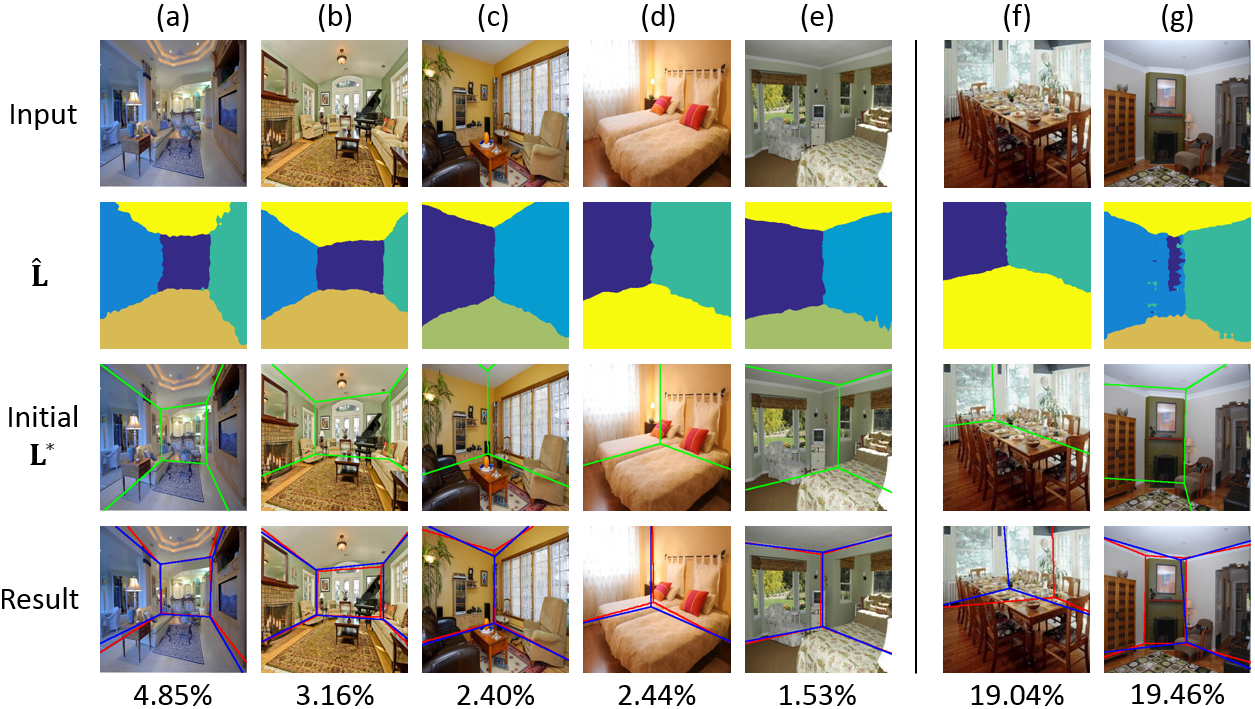
\includegraphics[width=8.5cm]{figure/qualitive.png}}
	\caption{Qualitative results and their pixel error of our method on LSUN validation set. Ground truth is shown in red. (a)-(e) depict precise results. (f)(g) show failure cases misled by $\vb{\hat{L}}$. }
	\label{fig:qualitative}
\end{figure}

\begin{table}
	\centering 
	\begin{tabular}{lcc}
		\toprule
		Method & $\epsilon_{corner}$ (\%) & $\epsilon_{pixel}$ (\%) \\
		\midrule
		Hedau et al.~\cite{hedau2009recovering} & 15.48 & 24.23 \\
		Mallya et al.~\cite{mallya2015learning} & 11.02 & 16.71 \\
		Zhang et al.~\cite{zhang2017learning} & 8.70 & 12.49 \\
		Dasgupta et al.~\cite{dasgupta2016delay} & 8.20 & 10.63 \\
		Ren et al.~\cite{ren2016coarse} & 7.95 & 9.31 \\
		Lee et al.~\cite{LeeRoomNet17} & 6.30 & 9.86 \\
		Zhao et al.~\cite{zhao2017physics} & 3.84 & 5.29 \\
		\midrule
		Proposed MC-FCN & 4.98 & 6.91 \\
		\bottomrule
	\end{tabular}
	\caption{Performance on the LSUN dataset~\cite{zhang2015large}.}	
	\label{table:comparison-lsun}
\end{table}

\subsection{Results on Hedau Dataset}
\label{sec:Hedau}
We also conduct experiments on the Hedau dataset \cite{hedau2009recovering}, which consists of 209 training images and 104 testing images. 
Since the semantic boundaries in the ground truth are thick and treated as a new category in this dataset, we perform boundary thinning to single pixel width by assigning them with the closest segmentation label, same as \cite{LeeRoomNet17}. We directly evaluate our method on the test set of Hedau  dataset using the model trained on LSUN. 
Pixel-wise error is adopted as the metric. 
As shown by Table~\ref{table:comparison-hedau}, our performance is better than \cite{mallya2015learning,zhang2017learning,ren2016coarse}, all of which are trained on the Hedau's training set. This indicates that our model has a good generalization ability. 
Our method achieves impressive performance on this dataset.

\begin{table}
	\centering 
	\begin{tabular}{lc}
		\toprule
		Method & $\epsilon_{pixel}$ (\%) \\
		\midrule
		Hedau et al.~\cite{hedau2009recovering} & 21.20 \\
		Mallya et al.~\cite{mallya2015learning} & 12.83 \\
		Zhang et al.~\cite{zhang2017learning} & 12.70 \\
		Dasgupta et al.~\cite{dasgupta2016delay} & 9.73 \\
		Ren et al.~\cite{ren2016coarse} & 8.67 \\
		Lee et al.~\cite{LeeRoomNet17} & 8.36 \\
		Zhao et al.~\cite{zhao2017physics} & 6.60 \\
		\midrule
		Proposed MC-FCN & \textbf{6.07} \\
		\bottomrule
	\end{tabular}
	\caption{Performance on the Hedau dataset~\cite{hedau2009recovering}. \comments{6.07 using the metric in \cite{LeeRoomNet17}, 7.90 using the metric in \cite{zhao2017physics}}}
	\label{table:comparison-hedau}
\end{table}



